 %%	SECCION documentclass																									 %%	
%%---------------------------------------------------------------------------%%
\documentclass[a4paper]{report}

%%---------------------------------------------------------------------------%%
%%	SECCION usepackage																											 %%	
%%---------------------------------------------------------------------------%%
\usepackage{amsmath, amsthm}
\usepackage[spanish,activeacute]{babel}
\usepackage{caratula}
\usepackage{a4wide}
\usepackage{hyperref}
\usepackage{fancyhdr}
\usepackage{graphicx} % Para el logo magico!
\usepackage{amssymb}
\usepackage{amsmath}
\usepackage[latin1]{inputenc}
%\usepackage [T1]{fontenc}
\usepackage[dvipsnames,usenames]{color}
\usepackage{amsfonts}
\usepackage{ulem}
%\usepackage{highlight}
\usepackage{fancybox}
%\usepackage{marvosym}
\usepackage{color}

%%---------------------------------------------------------------------------%%
%%	SECCION opciones																												 %%	
%%---------------------------------------------------------------------------%%
\parskip    = 11 pt
\headheight	= 13.1pt
\pagestyle	{fancy}
\definecolor{orange}{rgb}{1,0.5,0}

\addtolength{\headwidth}{1.0in}

\addtolength{\oddsidemargin}{-0.5in}
\addtolength{\textwidth}{1.0in}
\addtolength{\topmargin}{-0.5in}
\addtolength{\textheight}{0.7in}

%%---------------------------------------------------------------------------%%
%%	SECCION document	 %%	
%%---------------------------------------------------------------------------%%
\begin{document}
\renewcommand{\chaptername}{Parte }

%%---- Caratula -------------------------------------------------------------%%
\materia{Ingenier�a del Software II (2do cuatrimestre de 2009)}
\titulo{Trabajo Pr�ctico I - Primera Entrega}

\integrante{Castillo, Gonzalo}{164/06}{gonzalocastillo\_086@hotmail.com}
\integrante{Elizalde, Victoria}{452/06}{kivielizalde@gmail.com}
\integrante{Gonzalez, Sergio}{481/06}{gonzalezsergio2003@yahoo.com.ar}
\integrante{Page Saal, Mart�n}{315/06}{martinpage2001@yahoo.com.ar}
\resumen{
En el siguiente documento, se arribar� la fase de elaboraci�n del proyecto relacionado con la implementaci�n de un sistema de mediciones telem�tricas, que unir� puntos estrat�gicos del pa�s con el fin de capturar la informaci�n necesaria y procesarla, para anticiparse a los diferentes fen�menos meteorol�gicos. En dicha fase se identificar�n y detallar�n las funcionalidades principales del sistema y su arquitectura b�sica. Adem�s se definir� un plan detallado para esta primera iteraci�n del proyecto sin tener en cuenta la iteraci�n de de la fase de incepci�n ya dada por la c�tedra.}

% TOC, usa estilos locos
\maketitle
\pagestyle{empty}
{
\fancypagestyle{plain}
    {
    \fancyhead{}
    \fancyfoot{}
    \renewcommand{\headrulewidth}{0.0pt}
    } % clear header and footer of plain page because of ToC
\tableofcontents
}

\newpage
% arreglos los estilos para el resto del documento, y
% reseteo los numeros de pagina para que queden bien
\pagenumbering{arabic}
\fancypagestyle{plain} {
    \fancyhead[LO]{Castillo, Elizalde, Gonzalez, Page Saal}
    \fancyhead[C]{}
    \fancyhead[RO]{P\'agina \thepage\ de \pageref{LastPage}}
    \fancyfoot{}
    \renewcommand{\headrulewidth}{0.4pt}
}
\pagestyle{plain}

\newpage
\chapter{Introducci�n}

\section{Notaci�n}

Agregaremos unos pocos t�rminos nuevos que se utilizaran a lo largo de este documento. 

\begin{itemize}
	\item ECP : Estaci�n Central Provincial
	\item SMP : Sistema de Monitoreo Provincial
\end{itemize}

\section{Introducci�n}

En esta segunda parte del proyecto, nos encontramos con una serie de requerimientos, que son nuevos y que se agregan a los que se ten�an en la primera parte. Adem�s de esto, se contin�a con el crecimiento del proyecto con una metodolog�a diferente a la que se ven�a utilizando, esta metodolog�a es scrum, y como funciona de manera iterativa e incremental, adem�s de funcionar diferente a UP, se tuvo que adaptar a esta nueva forma de pensar el problema, e ir avanzando en el proyecto.

As� es de esta forma, en lo que sigue de este informe, se ver�n todas estas nuevas caracter�sticas, expuestas en las diferentes secciones. Para adaptarnos a los nuevos requerimientos, en la fase de planificaci�n, identificamos las funcionalidades mas importantes que tiene que tener el sistema y las agrupamos en epics. Vale aclarar que estas nuevas funcionalidades impulsaron un cambio en la arquitectura que se expuso anteriormente en la primera entrega, pero estos cambios no fueron tan graves. Tambi�n se realiz� el product backlog, y el sprint backlog con los user stories que se tienen que incluir seg�n lo pedido, con sus respectivas estimaciones, teniendo en cuenta la duraci�n del sprint que es de 2 semanas. Las etapas que se pusieron en pr�ctica son las siguientes:

\begin{itemize}

\item Planeamiento: En esta etapa se identificaron los nuevos requerimientos que se agregaron al sistema y se pusieron los epics relacionados. Tambi�n se realiz� el sprint backlog con los user stories que se corresponden con los nuevos requerimientos y los epics. Estos user stories son los que se espera que tenga el sistema al final cuando se termine.

\item Realizaci�n del sprint backlog: Aqui se tomaron los user stories que deben entrar para esta entrega, cada uno de estos fue estimado, estimando primeramente las tareas en las que fueron descompuestos cada uno, llegando a un consenso y luego en base a esto se asignaron esfuerzos a cada uno.

\item Casos de aceptaci�n: Algo que no estaba pedido en el enunciado expl�citamente, pero que nos pareci� correcto poner para agregar mas informaci�n en relaci�n a la finalizaci�n de cada user storie.


\end{itemize}

Luego de esto, se explican con detalle los cambios realizados a la arquitectura, donde surge el concepto de estaci�n central provincial (ECP), estaciones que estar�n en cada provincia, teniendo como funci�n principal, el procesamiento de los datos que le brindan las TRs de la zona, adem�s de la colaboraci�n con otras estaciones centrales, brind�ndoles informaci�n de su �rea como ser informaci�n de TRs, como resultados de los modelos.

Adem�s de lo mencionado anteriormente, se tuvo que realizar el dise�o de la secci�n relacionada con la ejecuci�n de los modelos matem�ticos, que en este caso, tiene que realizarse de forma distribuida. Para esto se hizo un dise�o, donde se detalla el funcionamiento que tendr� esta funcionalidad en el sistema. Dicho dise�o, es un diagrama de clases, y para describir el funcionamiento de la colaboraci�n de los objetos, se realiz� un diagrama de objetos y diversos diagramas de secuencia (de colaboraci�n). De esta forma queda bien explicado el funcionamiento de la ejecuci�n en forma distribuida de las reglas de un modelo, como se pide en el enunciado del trabajo.

Por �ltimo, se realiz� una comparaci�n entre el proceso de scrum y el proceso UP de desarrollo de sofware, donde incluimos opiniones al respecto.
\clearpage

\newpage
\chapter{Objetivo del sprint}

La caracter�stica principal de �ste sprint es la aparici�n de nuevos requerimientos funcionales.  Esto hace que se tenga que pensar como se adec�a la arquitectura a dichos requerimientos y en caso de ser necesario, c�mo deber�a modificarse para contemplar los mismos, teniendo en cuenta que funcione todo lo hecho hasta el momento. Entonces, b�sicamente el objetivo del sprint es adaptar la arquitectura pensada en la primera entrega del trabajo pr�ctico a los nuevos requerimientos, y llevar a cabo la nueva planificaci�n utilizando scrum. Una vez hecho esto debemos seleccionar la lista de stories que llevaremos a cabo en el sprint, estimarlos (utilizando valores relativos, que luego se traducir�n a esfuerzo) y comenzar con su implementaci�n para lograr un adecuado product increment que sea aceptado por el usuario.

Ser� necesario pensar c�mo van a impactar los nuevos requerimientos en la arquitectura ya dise�ada y como realizar un adecuado trade off para seguir garantizando el cumplimiento de los antiguos requerimientos y la satisfacci�n de los nuevos.

Tambi�n se espera tener los primeros stories realizados, que se corresponden con los que se indican en el enunciado del trabajo, resolviendo los problemas que surjan en el trayecto del mismo. Este avance se ver� reflejado en el Sprint Burndown Chart final, y se podr� observar como fue evolucionando el sprint durante las 2 semanas que dura.

Se espera fijar ademas las ideas cuando se tengan dudas acerca del proyecto su avance y su desarrollo cuando tengamos las stand-up meetings correspondientes, corroborando el seguimiento del proyecto.
\clearpage

\newpage
\chapter{Plan del Proyecto}

\section{Estimaciones a los casos de uso del proyecto(Asignaci�n de pesos)}

El m�todo que se utiliz� para estimar las tareas fue Wideband Delphi. A continuaci�n se detallar�n las principales etapas del proceso, sus complicaciones, resultados en com�n y las conclusiones finales.

\subsection{Planificaci�n y reuni�n de lanzamiento}

Estas dos etapas del proceso fueron b�sicamente, para poner en com�n que se iban a estimar los casos de uso de la secci�n anterior, el m�todo utilizado, y la medida que se iba a utilizar para la estimaci�n, en nuestro caso llegamos a que la medida para estimar viene dada por horas/persona. Esta decisi�n fue tomada m�s que nada para simplificar la estimaci�n y no tener que trabajar en horas en esta parte del proyecto. El objetivo b�sico de �stas estimaciones fue para poder luego determinar cantidad de iteraciones, duraci�n y fase a la que pertenecen de manera m�s o menos objetiva. Los encargados de llevar a cabo las estimaciones fuimos los 4 integrantes del grupo.

\subsection{Preparaci�n individual y reuni�n de estimaci�n}

En estas dos etapas del proceso llevamos a cabo cada una de las estimaciones que consideramos necesarias para cada uno de los casos de uso. Luego analizamos diferencias realizando gr�ficos que reflejaran la informaci�n de las estimaciones como se detalla a continuaci�n.

La primera ronda de estimaciones gener� los siguientes resultados:

\begin{figure}[H]
  \centering
    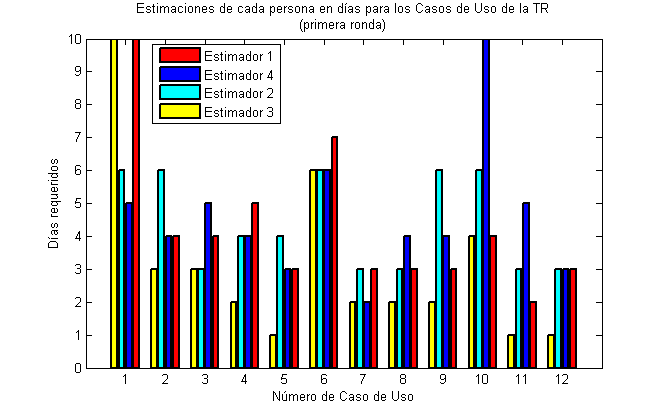
\includegraphics[scale=0.7]{EstimacionTR1raRonda.png}
\end{figure}

\begin{figure}[H]
  \centering
    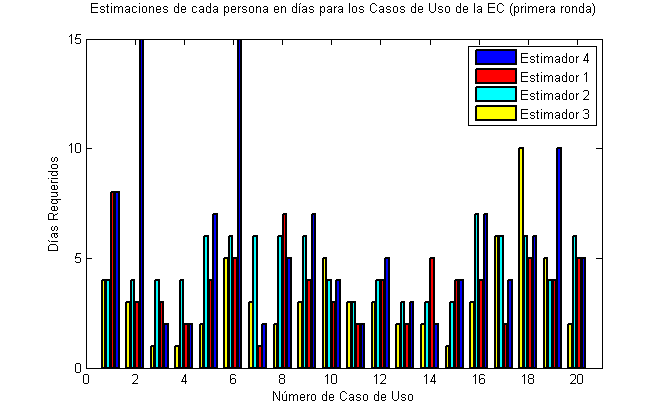
\includegraphics[scale=0.7]{EstimacionEC1raRonda.png}
\end{figure}

\begin{figure}[H]
  \centering
    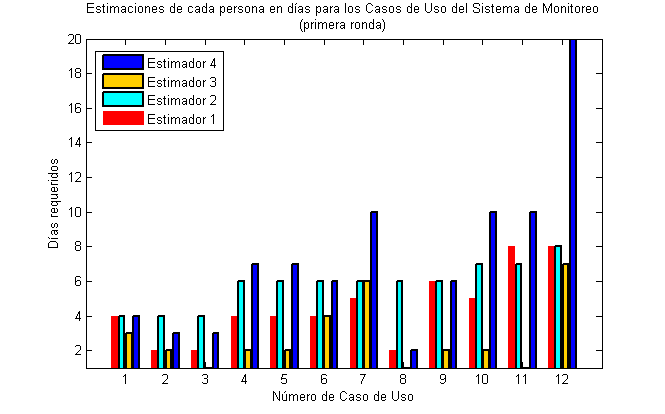
\includegraphics[scale=0.7]{EstimacionSM1raRonda.png}
\end{figure}

\clearpage
\newpage

Hab�a muchas tareas que difer�an bastante en la estimaci�n por lo cual en la primera reuni�n de estimaci�n se intent� nuevamente ver el alcance de cada caso de uso, lo cual sirvi� para que algunos estimadores pudieran tener en cuenta tareas y funcionalidades que en principio no hab�an considerado. Luego se procedi� a realizar una segunda ronda de estimaciones y los resultados se detallan a continuaci�n en los siguientes gr�ficos:

\begin{figure}[!Hb]
    \centering
    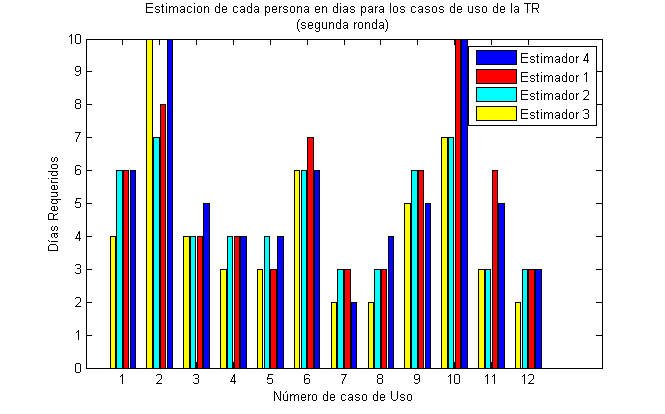
\includegraphics[width=13cm,height=7cm]{EstimacionTR2daRonda.png}
\end{figure}

\begin{figure}[!Hb]
    \centering
    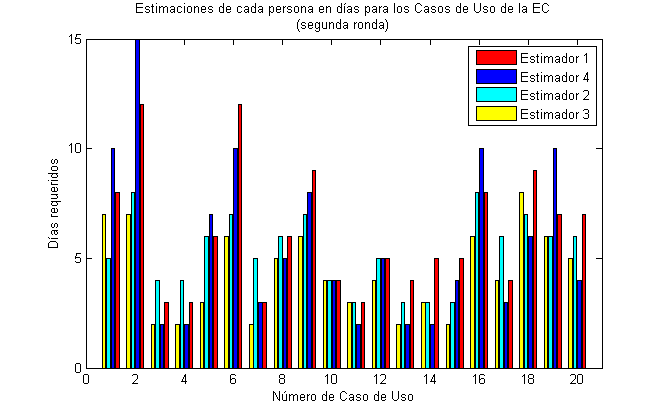
\includegraphics[width=13cm,height=7cm]{EstimacionEC2daRonda.png}
\end{figure}

\begin{figure}[!Hb]
    \centering
    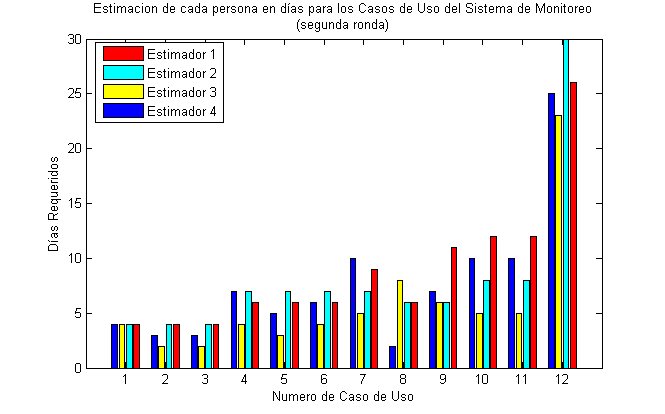
\includegraphics[width=13cm,height=7cm]{EstimacionSM2daRonda.png}
\end{figure}


\clearpage
\newpage

Si bien hubo mejor�as en la segunda ronda, consideramos que exist�an desv�os no aceptables, por lo cual nuevamente se revisaron los casos de uso y se lleg� a la conclusi�n que una tercera ronda de estimaciones reducir�a �stos desv�os. Luego de la tercera ronda consideramos detener las estimaciones ya que el desv�o fue aceptable (alrededor de dos d�as )y las estimaciones, calculando un promedio entre ellas pod�an llegar a reflejar valores adecuados. Los resultados son los siguientes: 

\begin{figure}[!Hb]
    \centering
    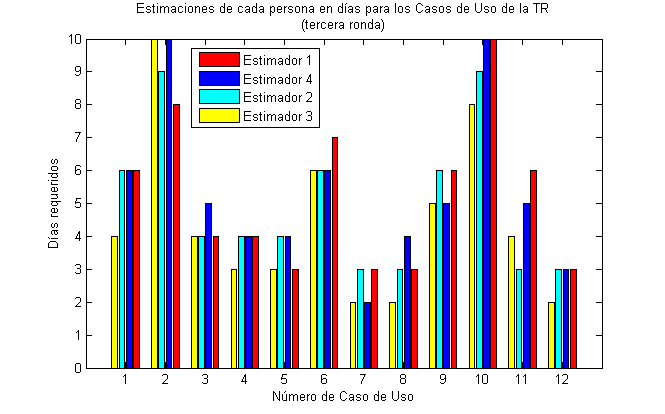
\includegraphics[width=13cm,height=7cm]{EstimacionTR3raRonda.png}
\end{figure}

\begin{figure}[!Hb]
    \centering
    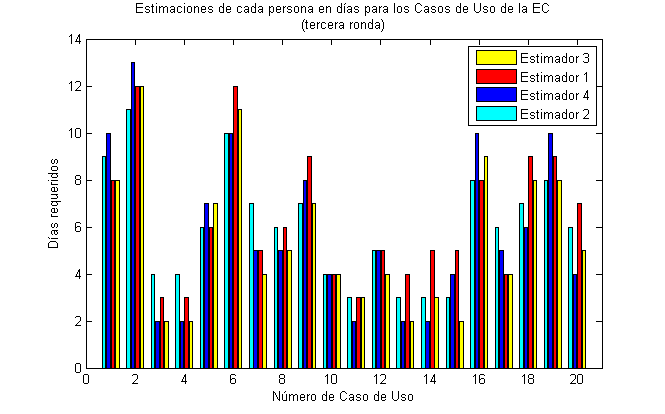
\includegraphics[width=13cm,height=7cm]{EstimacionEC3raRonda.png}
\end{figure}

\begin{figure}[!Hb]
    \centering
    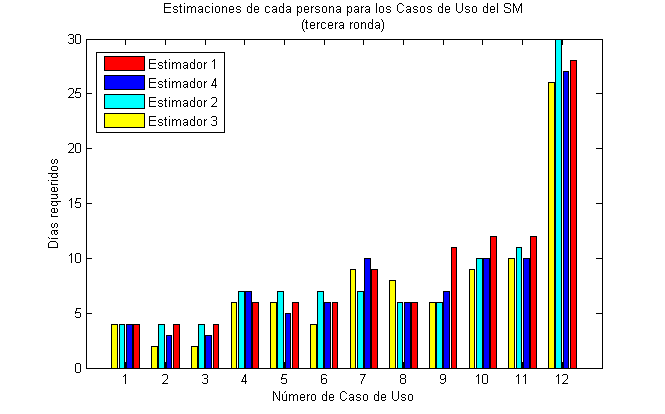
\includegraphics[width=13cm,height=7cm]{EstimacionSM3raRonda.png}
\end{figure}


\clearpage
\newpage
\subsection{Ensamblado de tareas y revisi�n de resultados}

Finalmente en �sta secci�n se calcul� un promedio de las estimaciones realizadas para cada tarea por cada estimador y se pudo concluir en resultados que a todos los integrantes le parecieron adecuados. A continuaci�n se detallan los pesos asignados a cada caso de uso que resultaron del proceso de estimaci�n.

\begin{itemize}

\item Casos de uso de la TR.
	
\begin{tabular}{||l | r||}
\hline
\hline
N�mero CU & Duraci�n en hs. (d�as) \\
\hline
 CU 1  & 120 (5) \\
\hline
 CU 2  & 216 (9) \\
\hline 
 CU 3  & 96 (4)\\
\hline
 CU 4  & 72 (3)\\
\hline
 CU 5  & 72 (3)\\
\hline
 CU 6  & 144 (6)\\
\hline
 CU 7  & 48 (2)\\
\hline
 CU 8  & 72 (3)\\
\hline
 CU 9  & 120 (5)\\
\hline
 CU 10  & 216 (9)\\
\hline
 CU 11  & 96 (4)\\
\hline
 CU 12  & 48 (2)\\
\hline
\hline
\end{tabular}
\newline

\item Casos de uso de la EC.
	
\begin{tabular}{||l | r||}
\hline
\hline
N�mero CU & Duraci�n en hs. \\
\hline
 CU 1  & 192 (8)\\
\hline
 CU 2  & 288 (12)\\
\hline 
 CU 3  & 48 (2)\\
\hline
 CU 4  & 48 (2)\\
\hline
 CU 5  & 144 (6)\\
\hline
 CU 6  & 240 (10)\\
\hline
 CU 7  & 120 (5)\\
\hline
 CU 8  & 120 (5)\\
\hline
 CU 9  & 168 (7)\\
\hline
 CU 10  & 96 (4)\\
\hline
 CU 11  & 48 (2)\\
\hline
 CU 12  & 96 (4)\\
\hline
 CU 13  & 48 (2)\\
\hline
 CU 14  & 72 (3)\\
\hline
 CU 15  & 72 (3)\\
\hline
 CU 16  & 192 (8)\\
\hline
 CU 17  & 96 (4)\\
\hline
 CU 18  & 168 (7)\\
\hline
 CU 19  & 192 (8)\\
\hline
 CU 20  & 120 (5)\\
\hline
\hline
\end{tabular}
\newline

\item Casos de uso del SM.
	
\begin{tabular}{||l | r||}
\hline
\hline
N�mero CU & Duraci�n en hs. \\
\hline
 CU 1  & 96 (4)\\
\hline
 CU 2  & 72 (3)\\
\hline 
 CU 3  & 72 (3)\\
\hline
 CU 4  & 144 (6)\\
\hline
 CU 5  & 144 (6)\\
\hline
 CU 6  & 120 (5)\\
\hline
 CU 7  & 192 (8)\\
\hline
 CU 8  & 144 (6)\\
\hline
 CU 9  & 168 (7)\\
\hline
 CU 10  & 240 (10)\\
\hline
 CU 11  & 240 (10)\\
\hline
 CU 12  & 648 (27)\\
\hline
\hline
\end{tabular}

\end{itemize}

\subsection{Armado de planificaci'on de iteraciones}

A partir de los resultados anteriormente obtenidos se realiz� una estimaci'on global del proyecto, conjuntamente con la divisi'on en iteraciones y la asignaci'on de los casos de uso a las distintas iteraciones

\begin{itemize}
	\item Inception 01 - Resuelta por los docentes de ISII
	\item Elaboration 01 - Iteraci'on actual - Casos de uso asociados a la primera iteraci�n, documento con las secciones correcpondientes detalladas en los entregables de la primera iteraci�n(Riesgos, Arquitectura, Atributos de Calidad, Prueba de concepto, etc)
	\item Elaboration 02 - Refinamiento final de casos de uso y definici�n de algunos protocolos cr�ticos
	\item Construction 01 - TR10, TR11, TR12, EC12, EC13, EC18 (lo que no se lleg� a hacer en Elab. 1 y 2)
	\item Construction 02 - TR01, TR02, TR04, TR05, TR06
	\item Construction 03 - TR03, TR07, TR08, TR09, EC01, EC10
	\item Construction 04 - EC05, EC06, EC07, EC08
	\item Construction 05 - EC02, EC03, EC04, EC11, EC15, EC17
	\item Construction 06 - EC09, EC14, EC20, SM01, SM02, SM03
	\item Construction 07 - EC16, EC17, SM06, SM08
	\item Construction 08 - SM04, SM05, SM07, SM09
	\item Construction 09 - SM10, SM11
	\item Construction 10 - SM12
	\item Transition 01 - Puesta en producci�n y test integral
	\item Transition 02 - Puesta en producci�n y test integral
	\item Transition 03 - Puesta en producci�n y test integral
\end{itemize}

Se debe destacar que el orden elegido para realizar los casos de uso se debio a partes cr�ticas del sistema y se priorizo entonces en este orden: protocolo, sensores, datos, ca�das, procesos matem�ticos, energ�a de TR, y luego el resto de las tareas.

Es tambi�n pertinente que en cada etapa de construcci�n se realicen los test de integraci�n posibles con los casos de usos ya realizados en las iteraciones anteriores.

El tiempo de las iteraciones de construcci�n es de un mes mientras que las de elaboraci�n son de 5 semanas y las de transici�n de 3 lo que da un costo total del proyecto en tiempo de aproximadamente 60 semanas.

\clearpage
\newpage

\section{Planificaci�n de la primera iteraci�n}

En esta parte del informe se mostrar�n todos los procedimientos llevados a cabo para obtener una completa y consistente  planificaci�n de la primera iteraci�n. Finalizadas dichas etapas se presentar� el diagrama Gantt resultante de la recopilaci�n de todos los datos de la planificaci�n. 

\subsection{Divisi�n en tareas de los casos de uso para la primera iteraci�n}

En esta secci�n consideraremos las tareas asociadas a los casos de uso que fueron determinados para la primera iteraci�n por la c�tedra. Cabe destacar que s�lo se van a considerar un subconjunto de las tareas para cada caso de uso, ya que constituyen una prueba de concepto y la funcionalidad completa se podr� completar en el resto de las iteraciones.

\subsubsection{Casos de uso asociados a la terminal remota}

\begin{enumerate}
  \item Sincronizando datos de censados. (TR09)

	\begin{itemize}
			\item Investigaci�n
		\begin{itemize}
			\item Posibles formar de completar datos seg�n m�todos num�ricos.
			\item Librer�as de alarmas y precisi�n de las mismas(deben tener en cuenta el tiempo REAL que paso y no solo el que tardo la aplicaci�n en ejecutar).
		\end{itemize}
		\item Implementaci�n
			\begin{itemize}
			\item Verificador de datos completos.
			\item Completador de datos seg�n datos hist�ricos.
			\item Armador de paquete de datos.
			\end{itemize}
		\item Testing
		 \begin{itemize}
		 \item Armado de datos falsos con posibles datos faltantes. 
		 \item Testing de unidad.
		 \end{itemize}
		\item Otros
      \begin{itemize}
      \item Armado de sandboxes para realizar implementaci�n.
       \item Generaci�n de datos falsos.
			\end{itemize}	
\end{itemize}

\item Encriptando/comprimiendo datos y enviado seg�n protocolo. (TR10)
\begin{itemize}
\item Investigaci�n
\begin{itemize}
\item Protocolo seguro y confiable para la TR con la EC.
\item Modelos de encriptaci�n/compresi�n de datos (NO para esta iteraci�n)
\end{itemize}
\item Implementaci�n
\begin{itemize}
\item Interfaz de capa de encriptaci�n/compresi�n de datos.
\item Capa de env�o de datos segura y confiable.
\end{itemize}
\item Testing
\item Otros
\begin{itemize}
\item Definir forma de generar datos falsos que luego puedan ser levantados por la EC.
\end{itemize}
\end{itemize}

\item Repitiendo mensaje si no llega confirmaci�n. (TR11)
\begin{itemize}
\item Investigaci�n
\begin{itemize}
	\item Formas de protocolos que permiten reenv�o de mensajes.
	\item Definir el tiempo esperado para el ACK.
\end{itemize}
\item Implementaci�n
\begin{itemize}
	\item Obtenci�n de dato anteriormente enviado sin ACK recibido.
	\item Protocolo de no reenv�o dato si llega alg�n ACK de todos los enviados.
\end{itemize}
\item Testing
\item Otros
\begin{itemize}
	\item Generaci�n de ACK falsos con probabilidad de arribo.
\end{itemize}
\end{itemize}

\item Borrando mensaje al llegar confirmaci�n. (TR12) 
\begin{itemize}
\item Implementaci�n
\begin{itemize}
	\item Buffer de datos hist�ricos ya enviados.
	\item Verificador de existencia de datos y sacarlo.
\end{itemize}
\item Testing
\begin{itemize}
	\item Generaci�n de datos falsos los cual ser�n los borrados luego.
\end{itemize}
\end{itemize}
\end{enumerate}

\subsubsection{Casos de uso asociados a la Estaci�n central}

\begin{enumerate}

\item Procesando modelos matem�ticos. (EC02)
\begin{itemize}
\item Investigaci�n
\begin{itemize}
	\item Modelos matem�ticos m�s simples para primera etapa.
\end{itemize}
\item Implementaci�n
\begin{itemize}
	\item Modelos Matem�ticos simples.
	\item Simulador de pedido de procesamiento de datos (Ya que no se hace CU1).
\end{itemize}
\item Testing
\item Otros
\begin{itemize}
	\item Armado del entorno que permita procesamiento de modelo.
\end{itemize}
\end{itemize}

\item Detectando ca�da/alta de TR. (EC05)
\begin{itemize}
\item Investigaci�n
\begin{itemize}
	\item Motivos de ca�da de una TR y formas de detecci�n.
\end{itemize}
\item Implementaci�n
\begin{itemize}
	\item Capa de detecci�n de ca�da por los casos antes mencionados.
	\item Verificador real de que la TR de que la esta ca�da.
	\item Regenerarador de TR original al detectar alta.
\end{itemize}
\item Testing
\begin{itemize}
	\item Armado de escenario falsos simulando ca�da de TR.
\end{itemize}
\end{itemize}
\item Ordenando/descartando mensajes repetidos. (EC12)

\begin{itemize}
\item Investigaci�n
\begin{itemize}
	\item Protocolos de descarte de SMS y formas de darse cuenta de dicho caso.
\end{itemize}
\item Implementaci�n
\begin{itemize}
	\item Almacenamiento de mensajes hist�ricos para verificar si es repetido.
  \item Etiquetador �nico para mensaje.
\end{itemize}
\item Testing
\begin{itemize}
	\item Armado de ambiente para simular mensajes repetidos
\end{itemize}
\end{itemize}

\item Confirmando llegada de mensaje. (EC13)

\begin{itemize}
\item Investigaci�n
\begin{itemize}
	\item 
Formato de ACK e informaci�n extra que pueda ser �til enviar (como un identificador �nico de error).
\end{itemize}
\item Implementaci�n
\begin{itemize}
	\item Recibidor de mensaje.
	\item Verificador de mensaje correcto.
	\item Capa (simple) de desencriptaci�n / descompresi�n. 
	\item Env�o de mensaje con ACK.
\end{itemize}
\item Testing
\begin{itemize}
	\item Generaci�n de mensajes falsos para poder simular recibirlos y confirmar.
\end{itemize}
\end{itemize}

\item Recibiendo, descomprimiendo y desencriptando mensaje de TR. (EC18)

\begin{itemize}
\item Investigaci�n
\begin{itemize}
	\item Formato de datos a recibir.
\end{itemize}
\item Implementaci�n
\begin{itemize}
	\item Capa de recibo de mensajes (ver CU anterior).
\end{itemize}
\item Testing
\begin{itemize}
	\item Generar datos falsos para poder recibir.
\end{itemize}
\end{itemize}


\end{enumerate}


\subsection{Estimaci�n, duraci�n de tareas asociadas a la primera iteraci�n}

En principio, lo que se hizo en �sta etapa es, como resultado de la divisi�n en subtareas para llevar a cabo la prueba de concepto, reducir considerablemente los tiempos estimados de dichos casos de uso, ya que la funcionalidad completa no era necesaria a esta altura del proyecto, sino que las funcionalidades a implementar se corresponden con un conjunto minimal de dichos casos de uso. Entonces luego de una evaluaci�n y puesta en com�n de todos los integrantes del grupo se lleg� a la conclusi�n que el tiempo que se necesita para implementar ese conjunto de funcionalidades para cada caso de uso es el siguiente:

\begin{tabular}{||l | r||}
\hline
\hline
N�mero CU & Duraci�n( En d�as/persona de 6 horas) \\
\hline
 TR09  & 2 \\
\hline
 TR10  & 3 \\
\hline 
 TR11  & 2 \\
\hline
 TR12  & 2 \\
\hline
 EC02  & 2 \\
\hline
 EC05  & 3 \\
\hline
 EC12  & 2 \\
\hline
 EC13  & 1 \\
\hline
 EC18  & 3 \\
\hline
\hline
\end{tabular}

Estos tiempos corresponden a la implementaci�n de todas las subtareas mencionadas en la etapa anterior para los casos de uso abarcados en �sta iteraci�n.
Tambi�n se consideraron en las estimaciones presentadas en la tabla anterior los tiempos asociados a la instalaci�n de entornos de desarrollo para dichos casos de uso.

\subsection{Generaci�n de dependencias}

Luego lo que se hizo a partir de �stos casos de uso fue analizar dependencias entre s�. Se tuvieron en cuenta dependencias en cuanto a implementaciones necesarias para llevar a cabo otras, es decir del estilo: No voy a poder implentar este caso de uso a menos que tenga �stos otros dos implementados. Sin embargo como se ver� mas adelante en el Gantt realizado nos surgieron dependencias por falta de recursos. 

\subsection{Definici�n y asignaci�n de recursos}

Los 4 recursos que se utilizar�n son los cuatro integrantes del grupo cumpliendo cualquiera de los posibles roles como ser programador, analista de requerimientos, testers, etc. En general hubo muchas tareas en las cuales decidimos participar �ntegramente todos y otras en las cuales hacerlas en paralelo dividiendo recursos nos era m�s ventajoso ya que los tiempos se acortaban considerablemente.

\subsection{Estimaci�n y precedencias en el resto de las tareas del proyecto y generaci�n de diagrama Gantt}

En esta secci�n vamos a describir brevemente el armado del diagrama Gantt correspondiente a la planificaci�n de la primera iteraci�n. Adem�s de las tareas asociadas a los casos de uso mencionadas anteriormente (para la prueba de concepto), en el proyecto se tuvieron en cuenta todas las tareas asociadas a la primera iteraci�n tales como an�lisis de requerimientos, an�lisis de riesgo, definici�n de arquitectura e incluso las tareas que conllevaron a la planificaci�n y el armado del Gantt propiamente dicho.

Muchas de �stas tareas se estimaron de manera sencilla, o bien porque ya las hab�amos hecho antes de dise�ar el Gantt o bien porque en trabajos pr�cticos de otras materias hab�amos realizado tareas similares. Sin embargo tuvimos que hacer estimaciones sin muchos argumentos para aquellas tareas en las que en principio no conocemos un tiempo para realizarlas, tales como el armado de la arquitectura. De todos modos intentamos ser lo m�s realistas posibles en las estimaciones y dentro de lo posible cumplir con el cronograma y las fechas de entrega de cada parte del proyecto.

En el Gantt que se ver� en la siguiente secci�n, se podr�n observar tareas generales, precedencias por recursos o funcionalidad, tareas cr�ticas e incluso tres hitos que propusimos: fin de la preentrega, fin de la arquitectura y fin de la primera iteraci�n. Cabe destacar que las tareas asociadas a generaci�n de documentos de preentrega o entrega de primera iteraci�n corresponden a armar finalmente dicho documento para entregarlo. Sin embargo no corresponde a realizarlo en su totalidad, sino que el documento se realizar� en paralelo a medida que se avanza en el proyecto y lo que �sta tarea refleja es el armado, juntada de partes y revisiones finales. 

Es importante destacar que el calendario que utilizamos son los d�as de la semana incluyendo los s�bados y domingo ya que en realidad utilizaremos estos dias, por lo cual aproximamos que desarrollaremos tareas relacionadas con el proyecto alrededor de 6 horas por cada uno de los d�as mencionados anteriormente.

\subsection{Diagrama de Gantt}

A continuaci�n se presentar� el diagrama de Gantt finalmente concluido.

\newpage
\begin{figure}[H]
    \centering
    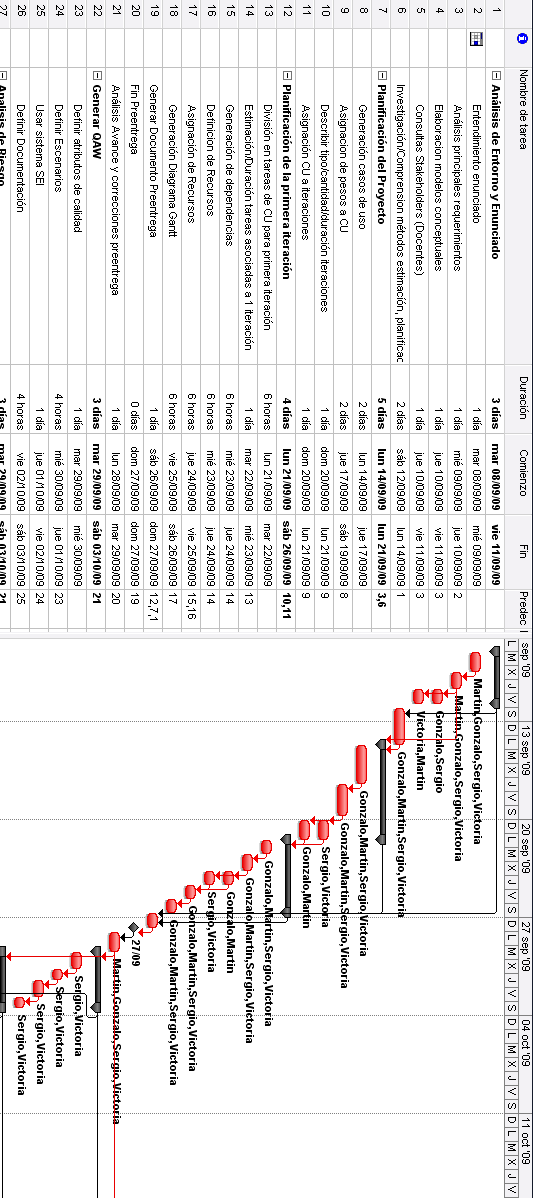
\includegraphics[scale = 0.6]{Gantt1E.png}
\end{figure}

\begin{figure}[H]
    \centering
    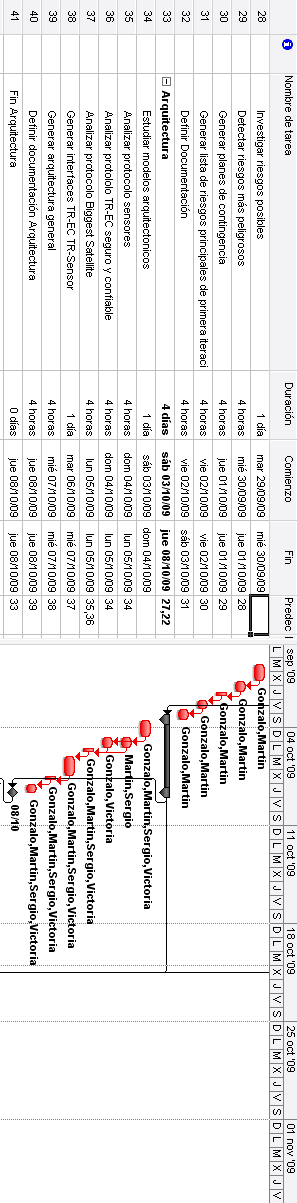
\includegraphics[scale = 0.6]{Gantt2aE.png}
\end{figure}

\begin{figure}[H]
    \centering
    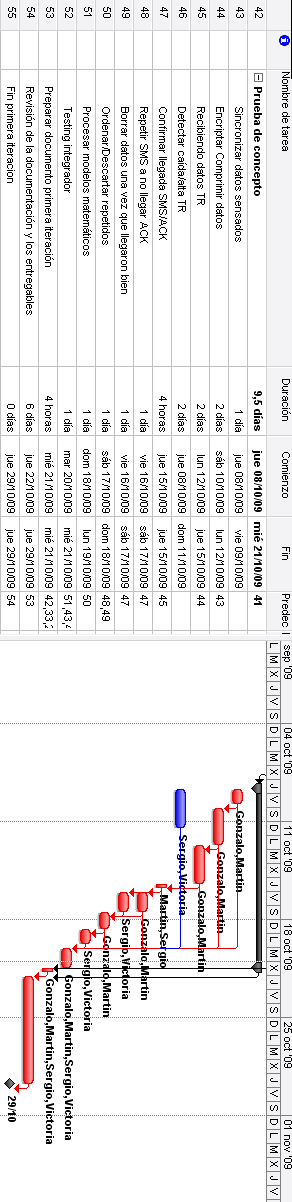
\includegraphics[scale = 0.6]{Gantt2bE.png}
\end{figure}
\clearpage

\section{Evaluaci�n, seguimiento y ajustes a la preentrega}

Una vez finalizada la planificaci�n detallada de la primera iteraci�n y el plan general del proyecto respresentados en lo que fue la preentrega del proyecto y llevada a cabo una primera validaci�n con stakeholder dada por la correci�n de la preentrega por nuestro corrector, se pudieron sacar en claro algunas conclusiones.

\begin{itemize}

\item Estimaciones: Pese a que era nuestra primera experiencia en estimaciones de tiempo y esfuerzo la utilizaci�n del m�todo Wideban Delphi no orient� bastante a la hora de estimar. Las cosultas post-entrega con los docentes y otros grupos rectificaron que la duraci�n total del proyecto entaba dentro de los l�mites pensados por la c�tedra. Adem�s se pudo seguir el cronograma detallado en el Gantt sin mayores complicaciones y finalmente entregar a tiempo la preentrega.
\item M�tricas de estimaci�n: En esta secci�n tuvimos que corregir algunas cuestiones que hac�a que el entendimiento de las estimaciones fuese complicado para nuestro corrector, es decir, si bien la informaci�n era consistente (el mismo corrector prob� un par de equivalencias) la informaci�n no era del todo clara y las m�tricas utilizadas eran diferentes de acuerdo a la parte del informe que llev�bamos a cabo. Por lo cual se ajustaron las m�tricas normaliz�ndolas para un mejor entendimiento de las mismas.
\item Gantt: El cronograma detallado en el Gantt hab�a quedado en d�as de 8 horas para compensar la no utilizaci�n de s�bados y domingos. Cambiamos �sto y preferimos utilizar los s�bados y domingo y d�as de 6 horas ya que se adapta mucho mejor a lo que se har� en realidad. Adem�s cada una de las funcionalidades que se muetran en el Gantt en la secci�n prueba de concepto se corresponden con la planificaci�n, dise�o, implementaci�n, armado de entornos de desarrollo y testing. Se agreg� adem�s la semana adicional dada por la c�tedra para completar el trabajo pr�ctico.
\item Eliminaci�n de un caso de uso: En la primera iteraci�n contemplabamos para la prueba de concepto el caso de uso asociado a la triangulaci�n, sin embargo posteriormente se determin� que dicha funcionalidad no era necesaria, por lo cual la quitamos de dicha iteraci�n.
\item Otros: Se corrigi� informaci�n mal redactada y otros detalles menores mencionados por el corrector. 
\end{itemize}


\clearpage

\newpage
\chapter{Gesti�n de riesgos}

En esta secci�n se discutir�n los riesgos m�s relevantes en el contexto de nuestro problema. Para cada uno de ellos definiremos las caracter�sticas que los definen incluyendo la probabilidad de que ocurran, el impacto (negativo) si ocurren (en una escala del 1 al 10), la exposici�n al riesgo (medida como probabilidad * impacto). Adem�s incluiremos en los casos que sea posible, formas de mitigarlo y tambi�n posibles planes de contingencia en caso de que ocurriesen.

\section{Identificaci�n de riesgos}

Para llevar a cabo la identificaci�n de riesgos tuvimos en cuenta en mayor o menor menor medida los siguientes m�todos:

\begin{itemize}

\item Brainstorm.
\item Cuestionario de identificaci�n taxon�mica.
\item Lista de riesgos comunes.

\end{itemize}

Para determinar la probabilidad de impacto y exposici�n al riesgo, primero determinamos los riesgos y luego cada uno estim� por separado estos valores (para no influirnos entre nosotros) y en base a esto discutimos despu�s y consensuamos los valores finales.

Finalmente los riesgos determinados fueron:

\begin{enumerate}

\item - R1 - Incorporar modelos matem�ticos err�neos.

\begin{itemize}
\item Probabilidad: 0.2
\item Impacto: 10
\item Exposici�n al riesgo: 2.0
\item Mitigaci�n: Hacer pruebas con los modelos antes de de ponerlos en funcionamiento. Probarlos con datos hist�ricos reales y ver si acierta las predicciones. Estas pruebas deber�an hacerse en conjunto con el meteor�logo que desarrollo el modelo para que pueda corregir eventuales errores.
\item Plan de Contingencia: Volver al �ltimo modelo matem�tico v�lido.
\end{itemize}

\textbf{En caso de:} incorporar modelos matem�ticos inexactos posiblemente se hagan predicciones incorrectas, lo cual es grav�simo en el contexto de nuestro sistema.
\item - R2 - Mala interpretaci�n de requerimientos no esenciales.

\begin{itemize}
\item Probabilidad: 0.3
\item Impacto: 6
\item Exposici�n al riesgo: 1.8
\item Mitigaci�n: Mayor tiempo de validaci�n con los stakeholders.
\item Plan de Contingencia: Solucionar de alguna manera, en tiempo de ejecuci�n los problemas generados.
\end{itemize}

\textbf{En caso de:} una mala interpretaci�n de los requerimientos no esenciales (aquellos no necesariamente cr�ticos) los usuarios no estar�n conformes y el posiblemente haya que corregir dichos errores despu�s de haber puesto el proyecto en producci�n.

\item - R3 - Infiltraci�n en modelo e�lico.

\begin{itemize}
\item Probabilidad: 0.1
\item Impacto: 6
\item Exposici�n al riesgo: 0.6
\item Mitigaci�n: --
\item Plan de Contingencia: Utilizar los datos generados por nuestro sistema aunque no sean m�s precisos que los del sistema e�lico.
\end{itemize}

\textbf{En caso de:} infiltraci�n en el modelo e�lico llegar�n datos incorrectos lo cual producir�, en caso de ser considerados v�lidos, resultados y reportes incorrectos de nuestro sistema.

\item - R4 - Quiebra de empresas que previamente hayan contratado nuestros servicios.

\begin{itemize}
\item Probabilidad: 0.09
\item Impacto: 7
\item Exposici�n al riesgo: 0.63
\item Mitigaci�n: Cobrar por adelantado los costos de la instalaci�n f�sica.
\end{itemize}

\textbf{En caso de:} Quiebre de empresas que previamente nos hayan contratado y se hayan instalado las componentes solicitadas los gastos de instalaci�n perjudicar�an la econom�a de la empresa. Para evitar esto, se deber�a cobrar por adelantado a la empresa siempre que sea posible.

\item - R5 - Ca�da p�gina de la infraestructura.

\begin{itemize}
\item Probabilidad: 0.4
\item Impacto: 4
\item Exposici�n al riesgo: 1.6
\item Mitigaci�n: Analizar con la infraestructura la posibilidad de que el mantenimiento del sitio web sea por parte de la empresa.
\item Plan de Contingencia: En caso de recuperaci�n tard�a crear una p�gina simple y temporal que provea nuestros servicios.
\end{itemize}

\textbf{En caso de:} Ca�da de la p�gina de la infraestructura los usuarios no podr�n acceder a la informaci�n provista por el sistema.

\item - R6 - Ca�da del servidor web (Alarmas).

\begin{itemize}
\item Probabilidad: 0.3
\item Impacto: 5
\item Exposici�n al riesgo: 1.5
\item Mitigaci�n: Estudiar, analizar e investigar el servidor que garantice mayor disponibilidad.
\item Plan de Contingencia: Utilizar alg�n tipo de sistema v�a sms para informar a los usuarios.
\end{itemize}

\textbf{En caso de:} ca�da del servidor web no podr� alertarse a los empleados de problemas como congesti�n o ca�das de TRs con lo cual habr�a que implementar alg�n tipo de interfaz alternativa que utilice mensajes de texto.

\item - R7 - Desarrollo de proyecto centralizado.

\begin{itemize}
\item Probabilidad: 0.1
\item Impacto: 6
\item Exposici�n al riesgo: 0.6
\item Mitigaci�n: Imponer pautas a cumplir por cada uno de los encargados del proyecto para evitar centralizaci�n.
\item Plan de Contingencia: Incrementar tiempo de proyecto.
\end{itemize}

\textbf{En caso de:} centralizaci�n del proyecto el mismo tender� a desarrollare en m�s tiempo.

\item - R8 - Incremento de requerimientos en tiempo de construcci�n.

\begin{itemize}
\item Probabilidad: 0.5
\item Impacto: 5
\item Exposici�n al riesgo: 2.5
\item Mitigaci�n: Planificar lo mejor que se pueda de manera pesimista.
\item Plan de Contingencia: Negarlos, en caso de no ser posible llevarlos a cabo pero intentando convencer a los stakeholders de un cierto incremento en el tiempo de entrega.
\end{itemize}

\textbf{En caso de:} incremento de los requerimientos el tiempo de desarrollo del proyecto se ver� necesariamente en aumento.

\item - R9 - Baja en los recursos.

\begin{itemize}
\item Probabilidad: 0.1
\item Impacto: 9
\item Exposici�n al riesgo: 0.9
\item Mitigaci�n: --
\item Plan de Contingencia: Incrementar tiempo de proyecto / incorporar nuevo recurso.
\end{itemize}

\textbf{En caso de:} una posible baja de alguno de los recursos que llevan a cabo el proyecto, el tiempo de desarrollo en el mismo tender� a incrementarse.

\item - R10 - Mal funcionamiento de la CMUM (Componente muy usada en el mercado).

\begin{itemize}
\item Probabilidad: 0.1
\item Impacto: 5
\item Exposicici�n al riesgo: 0.5
\item Mitigaci�n: --
\item Plan de Contingencia: Cambiar la componente.
\end{itemize}

\textbf{En caso de:} mal funcionamiento de la componente muy usada en el mercado para alguna TR, se puede producir la situaci�n de que la misma deje de funcionar, por lo cual hay que detectar la situaci�n r�pidamente y solucionar el problema.

\item - R11 - La arquitectura no satisface los requerimientos.

\begin{itemize}
\item Probabilidad: 0.4
\item Impacto: 9
\item Exposici�n al riesgo: 3.6
\item Mitigaci�n: Incrementar el tiempo dedicado a la arquitectura lo m�s que se pueda.
\item Plan de Contingencia: Solucionar los posibles problemas incrementalmente en tiempo de ejecuci�n.
\end{itemize}

\textbf{En caso de:} generar una mala arquitectura, se pueden producir muchos problemas posibles tales como lentitud en las conexiones, datos erroneos o inconsistentes, falta de disponibilidad, lo que har�a que nuestro software sea de mala calidad, con lo cual la idea es dedicarle el mayor tiempo posible validando en todo momento lo que se haya realizado. En todo caso se intentar� realizar una arquitectura flexible para que cualquier posible cambio se aplicable.

\item - R12 - Ca�da del servicio Biggest Satellite.

\begin{itemize}
\item Probabilidad: 0.2
\item Impacto: 8
\item Exposici�n al riesgo: 1.6
\item Mitigaci�n: --
\item Plan de Contingencia: cambiar el radio de triangulaci�n para generar TRs virtuales y calcular promedios con datos previos a la ca�da.
\end{itemize}

\textbf{En caso de:} ca�da del servicio Biggest Satellite en caso de necesidad de acceder a sus servicios por la ca�da de una TR y no poder triangular estar�amos dejando de proveer datos lo cual no puede suceder en nuestro sistema.

\item - R13 - Ca�da red GSM.

\begin{itemize}
\item Probabilidad: 0.05
\item Impacto: 10
\item Exposici�n al riesgo: 0.5
\item Mitigaci�n: Ninguna, la red GSM no depende de nosotros.
\item Plan de Contingencia: Utilizar el servicio Biggest Satellite a pesar de sus costos en conjunto con el sistema e�lico.
\end{itemize}

\textbf{En caso de:} ca�da de la red GSM nuestro proyecto es obsoleto.


\item - R15 - Uso de sensores que no soporten cifrado de la informaci�n enviada a las TRs.

\begin{itemize}
\item Probabilidad: 0.4
\item Impacto: 5
\item Exposici�n al riesgo: 2.0
\item Mitigaci�n: Informar a los stakeholders que tomen decisiones de que productos comprar, la necesidad de comprar sensores seguros.
\item Plan de Contingencia: Evaluar en el seguimiento del proyecto la idea de incrementar el tiempo de alguna de las iteraciones.
\end{itemize}

\textbf{En caso de:} utilizar sensores que se comunican en medios inseguros (Comunicaciones wireless, bluetooth, etc) y no cifren los datos que env�an, podr�a suceder que un intruso alterara los datos en vuelo (mediciones) antes de que lleguen a la TR y podamos detectarlo, tendr�amos datos incorrectos en el sistema y podr�amos arrojar pron�sticos (parcialmente) incorrectos.


\end{enumerate}

\section{Selecci�n de principales riesgos}

En esta secci�n usaremos una t�cnica provista por el SEI la cual consiste en armar una tabla, que nos permite, una vez armada nuestra lista de riesgos, clasificarlos seg�n 2 criterios: probabilidad y severidad de impacto. De esa forma, podremos determinar cuales son los riesgos mas severos que podr�an hacer fracasar nuestro proyecto.
En dicha tabla se ubicar� cada riesgo en su correspondiente celda de acuerdo al siguiente criterio:

En cuanto a probabilidad se clasificar�n en:

\begin{itemize}
\item Baja : menos de 0.3
\item Media : entre 0.3 y 0.6
\item Alta : mayor a 0.6
\end{itemize}

En cuanto a severidad se clasificar�n en:

\begin{itemize}
\item Marginal : menos de 3 
\item Normal : entre 3 y 6
\item Cr�tica : mayor a 6
\end{itemize}

A continuaci�n se podr�n observar cada uno de los riesgos mencionados en la secci�n anterior en la tabla.

\begin{tabular}{||l | c| c| c||}
\hline
\hline
Severidad/Probabilidad & Alta & Media & Baja\\
\hline
 Cr�tica  &  & R11, R14 & R1,R4,R9,R12,R13 \\
\hline
 Normal  &  & R8,R6,R2,R5 & R7,R10,R3,R15\\
\hline 
 Marginal &  &  & \\
\hline
\hline
\end{tabular}


Finalmente seleccionaremos los riesgos mas cr�ticos para nuestro proyecto. En base a la tabla, decidimos que los 2 riesgos m�s cr�ticos son R11 y R14, ya que son altamente probables y el riesgo de impacto es cr�tico. Luego, decidimos que el resto de los riesgos cr�ticos eran los que ten�an alta probabilidad o un impacto muy grande, es decir, dejamos de lado los riesgos R3, R7, R10 y R15.

Finalmente, nos pareci� que a los 2 riesgos mencionados antes, deber�amos agregar como cr�ticos los riesgos: R1, R5, R6 y R12 por un lado, y por otro R2, R8, R11 y R14. Los primeros 4 riesgos son riesgos que tendr�an como consecuencia no poder cumplir con el objetivo del sistema, ya se no poder realizar pron�sticos adecuados (1 y 5) o no poder alertar a la poblaci�n / los stakeholders de las amenazas (6 y 12). Por otro lado, est�n los riesgos que har�an fracasar nuestro proyecto de software desde el punto de vista del Plan de Proyecto (riesgos no espec�ficos al tema del proyecto, riesgos est�ndar que enfrenta un proyecto de software): no comprender los requerimientos correctamente, excederse en los plazos, no cumplir los atributos de calidad, es decir riesgos que hacen a la satisfacci�n del cliente.

Esta selecci�n se riesgos se hizo para reducir la lista y poder monitorear durante el resto del proyecto los riesgos cr�ticos para el proyecto, y concentrarse en ellos, rest�ndole algo de atenci�n a los menos cr�ticos (que sin embargo, tampoco ser�n dejados de lado por completo).

\section{An�lisis de los riesgos obtenidos}
Los riesgos encontrados pueden dividirse en dos categor�as: riesgos t�cnicos y riesgos de negocio. En su mayor�a son riesgos generales y no tan espec�ficos: esto responde a la etapa del proyecto en la que nos encontramos (es una etapa temprana, en la que se tiene una visi�n mas general o ``macro'' del proyecto). 

Si bien en la etapa de elaboraci�n suelen aparecer m�s que nada riesgos t�cnicos, es entendible que tambi�n hayan aparecido riesgos de negocio (que suelen aparecer en la fase de inception) ya que por un lado las disciplinas se superponen (que en la fase de elaboraci�n aparezcan riesgos t�cnicos no significa que sean los �nicos, ya que a veces aparecen espont�neamente algunos riesgos) y por otro porque el documento generado en la fase de Inception (el enunciado) no inclu�a un documento de gesti�n de riesgos.

Estamos contentos con los hacer utilizado mas de una t�cnica de identificaci�n de riesgos ya que se complementaron muy bien: debido a nuestra formaci�n acad�mica y profesional tenemos un sesgo t�cnico muy grande y es dif�cil que se nos ocurran riesgos de negocio / gesti�n, con lo cual leer cuestionarios y listas de riesgos comunes nos ayud� a tener una visi�n m�s completa.

Finalmente, hay que entender que este es solo un an�lisis de riesgos inicial, y que la gesti�n de riesgos tiene que seguir durante todo el proyecto. A medida que se avance en las diferentes etapas del proyecto, algunos riesgos desaparecer�n, y aparecer�n otros nuevos.
\clearpage

\newpage
\chapter{Conclusi�n}

Si bien se sabe que el dise�o del proyecto est� en sus primeros pasos, con lo realizado en esta preentrega, se tiene una especificaci�n relativamente exhaustiva de las cosas mas importantes del dominio del problema. Con estos datos se pudo definir la base de la arquitectura del sistema, que si bien puede cambiar, se supone que no afectara gravemente el dise�o original, ni traer� problemas que posterguen demasiado el proyecto.

Para realizar esta afirmaci�n nos basamos en que al realizar el diagrama contextual (que sirve en este caso de arquitectura), tomamos en cuenta varios de los requerimientos y atributos de calidad planteados inicialmente, proponiendo una arquitectura que es incremental, en cuanto a que se pueden agregar Terminales Remotas, y en cuanto a que se puede incrementar el poder de c�mputo. Tambi�n es resistente a fallas en las transmisiones, ya que se implementara un protocolo confiable entre las TRs y la Estaci�n Central y tambi�n es resistente a fallas en los equipos, dado que se van a poder subsanar la ca�da de una TR triangulando o utilizando un servicio externo. Adem�s se contempla el hecho de tener comunicaci�n con diferente tipo de sistemas, ya sean clientes externos (como AgroTop), proveedores de servicio (Biggest Satelite) y usuarios internos, encargados de monitorear el estado del sistema.

Se dise�� un plan que tiene en cuenta tiempos de entrega y de desarrollo que son acotados, por esta raz�n se tuvo que identificar dependencias entre las funcionalidades principales que se detectaron, como as� su importancia y complejidad dentro del sistema.

Como se conoce estos m�todos llevan bastante tiempo, pero ayudan a tener un control del proyecto y tener luego un hilo de ejecuci�n bien definido que permitir� optimizar el desarrollo del sistema durante el tiempo. Teniendo en cuenta el contexto en el que se realiz� el trabajo creemos haber cumplido las expectativas en cuanto a los requerimientos pedidos para esta entrega.

\clearpage
\label{LastPage}
\end{document}
